\documentclass[onecolumn,titlepage,letterpaper,10pt]{article}
\usepackage[letterpaper,margin=1in]{geometry}
\usepackage[affil-it]{authblk}
\usepackage{enumitem}
\setlist[itemize]{nosep, itemsep = 0pt, parsep=0pt, leftmargin = *, topsep = 0pt}
%parsep = 0pt,
%leftmargin = *,
%topsep = 0pt,
%}
\usepackage{subcaption}
\usepackage{import}
\usepackage{appendix}
\usepackage{setspace}
\usepackage[printwatermark]{xwatermark}
%\newwatermark[allpages,color=red!10,angle=90,scale=3.75,xpos=60,ypos=0]
%{DRAFT\textbullet DRAFT}
\usepackage{pdfpages}
%\pagenumbering{gobble}
\usepackage{multicol}
\usepackage{amsmath}
\usepackage[titletoc, toc, page]{appendix}
\usepackage{amsthm}
\newtheorem*{remark}{Remark}
\usepackage{mathtools}
%\mathtoolsset{showonlyrefs}
\usepackage{esint}
\usepackage{verbatim}
\usepackage{caption}
\usepackage{listings}
\lstset{
basicstyle=\small\ttfamily,
numbers=left,
numberstyle=\tiny,
frame=tb,
columns=fullflexible,
showstringspaces=true
}
%\usepackage{gensymb}
\usepackage{dirtytalk}
\usepackage{csquotes}
\usepackage{mathcomp}
\definecolor{blue}{cmyk}{1.0,0.44,0,0}
\usepackage[breaklinks=true,
colorlinks=true,
urlcolor=blue,
linkcolor=blue,
citecolor=blue]{hyperref}
\usepackage{url}
\usepackage{caption} %Allows for use of \caption* for non-labeled captions
\captionsetup{width = 0.7\textwidth}
\usepackage{graphicx}
\usepackage[section]{placeins}
\usepackage{lipsum}
\usepackage{booktabs}
\usepackage{tabularx}
\usepackage[textsize=tiny]{todonotes}
\usepackage{ltablex}
\usepackage{longtable}
\usepackage{titlesec}
\usepackage[numbers]{natbib}   % omit 'round' option if you prefer square brackets
\bibliographystyle{plainnat}
%%%%%%%%%%%%%%%%%%%%%%%%%%%%%%%%%%%%%%%%%%%%%%%%%%%%%%%%%%%%%%%%%%%%%%%%%%%%%%%%
% TIKZ STUFF
\usepackage{tikz}
\usetikzlibrary{shapes, arrows, decorations.markings,}
\usetikzlibrary{positioning}
% ------------------------------------------------------------------------------
% Define block styles
% ------------------------------------------------------------------------------
\tikzset{
    startstop/.style ={
        rectangle,
        rounded corners,
        minimum width=2cm,
        minimum height=1cm,
        text centered,
        thick,
        draw,
    },
    io/.style = {
        trapezium,
        trapezium left angle=70,
        trapezium right angle=110,
        text width=2cm,
        minimum height=1cm,
        align=center,
        thick,
        draw,
    },
    process/.style = {
        rectangle,
        text width=5cm,
        minimum height=1cm,
        align=center,
        thick,
        draw,
    },
    decision/.style = {
        diamond,
        text width=5cm,
        minimum height=1cm,
        align=center,
        thick,
        draw,
    },
}

\tikzstyle{arrow} = [thick,->,>=stealth]
%%%%%%%%%%%%%%%%%%%%%%%%%%%%%%%%%%%%%%%%%%%%%%%%%%%%%%%%%%%%%%%%%%%%%%%%%%%%%%%%
%% \usepackage{cite}
\graphicspath{ {images/} }
%% Custom Commands
\newcommand{\pprime}{^{\prime}}
\newcommand{\sn}[2]{#1\times10^{#2}}
\newcommand{\snu}[6]{#1\times10^{#2}\,^{+\sn{#3}{#4}}_{-\sn{#5}{#6}}}
\newcommand{\snuwo}[3]{#1\,^{+#2}_{-#3}}
\newcommand{\unitsb}[1]{\,[\text{#1}]}
\newcommand{\functionof}[2]{#1\left(#2\right)}
\newcommand{\CPP}
{C\nolinebreak[4]\hspace{-.05em}\raisebox{.22ex}{\footnotesize\bf ++\,}}

\newcommand*\widefbox[1]{\fbox{\hspace{2em}#1\hspace{2em}}}
\newcommand{\Lagr}{\mathcal{L}}
\newcommand{\ham}{\mathcal{H}}
\newcommand{\infinitesum}[2]{\sum_{#1 = #2}^{\infty}}
\newcommand{\goodprime}{^{\prime}}
\newcommand{\tsi}[1]{\int_{\phi=0}^{2\pi}\int_{\theta=0}^{\pi}\int_{r=0}^{#1}}
\newcommand{\unit}[1]{\,\hat{\bm{#1}}}
\newcommand{\units}[1]{\,\text{#1}}
\newcommand{\vect}[1]{\mathbf{#1}}
\newcommand{\paren}[1]{\left(#1\right)}
\newcommand{\brackets}[1]{\left[#1\right]}
\newcommand{\abs}[1]{\left|#1\right|}
\newcommand{\anglers}[1]{\langle #1 \rangle}
\newcommand{\sinp}[1]{\sin{\paren{#1}}}
\newcommand{\cosp}[1]{\cos{\paren{#1}}}
\newcommand{\tanp}[1]{\tan{\paren{#1}}}
\newcommand{\expp}[1]{\exp\paren{#1}}
\newcommand{\thefrac}{\dfrac{n\pi}{d}}
\newcommand{\assolegendre}[1]{P_{#1}\paren{\cos{\theta}}}
\newcommand{\kg}{\units{kg}}

\newcommand{\partialwoa}[1]{\dfrac{\partial}{\partial #1}}
\newcommand{\partialtop}[2]{\dfrac{\partial#1}{\partial #2}}
\newcommand{\partiald}[2]{\dfrac{\partial}{\partial #2}\brackets{#1}}
\newcommand{\partialdd}[2]{\dfrac{\partial^2}{\partial^2 #2}\brackets{#1}}
\newcommand{\derivative}[2]{\dfrac{d #1}{d #2}}
\newcommand{\integral}[2]{\int_{#1}^{#2}}

\newcommand{\onec}{\frac{1}{\degree\text{C}}}
\newcommand{\degrees}[1]{\,\degree\units{#1}}
\newcommand{\cunits}{\,\frac{\units{J}}{\units{kg}\cdot\degrees{C}}}
\newcommand{\idcunits}{\,\frac{\units{J}}{\units{mol}\cdot\text{K}}}
\newcommand{\idc}{8.3145\,\frac{\units{J}}{\units{mol}\cdot\text{K}}}
\newcommand{\firstlTD}{the First Law of Thermodynamics}


\newcommand{\theWorkingTitle}{Evolutionary Runge-Kutta}

\renewcommand\thesection{\arabic{section}}
%\setcounter{secnumdepth}{1}


\title{Honors Report\\
%\phantom{\_}\\
\large \theWorkingTitle\thanks{\url{https://github.com/jacksonlanecole/rkev}}}
\author{Jackson L. Cole}
\affil{Department of Physics and Astronomy, Middle Tennessee State University}
\date{Fall 2018}

\begin{document}
%%%%%%%%%%%%%%%%%%%%%%%%%%%%%%%%%%%%%%%%%%%%%%%
%% The following makes equations look much nicer
%% \setlength{\abovedisplayskip}{10pt}
%% \setlength{\belowdisplayskip}{10pt}
%% \setlength{\abovedisplayshortskip}{10pt}
%% \setlength{\belowdisplayshortskip}{10pt}
%%%%%%%%%%%%%%%%%%%%%%%%%%%%%%%%%%%%%%%%%%%%%%%
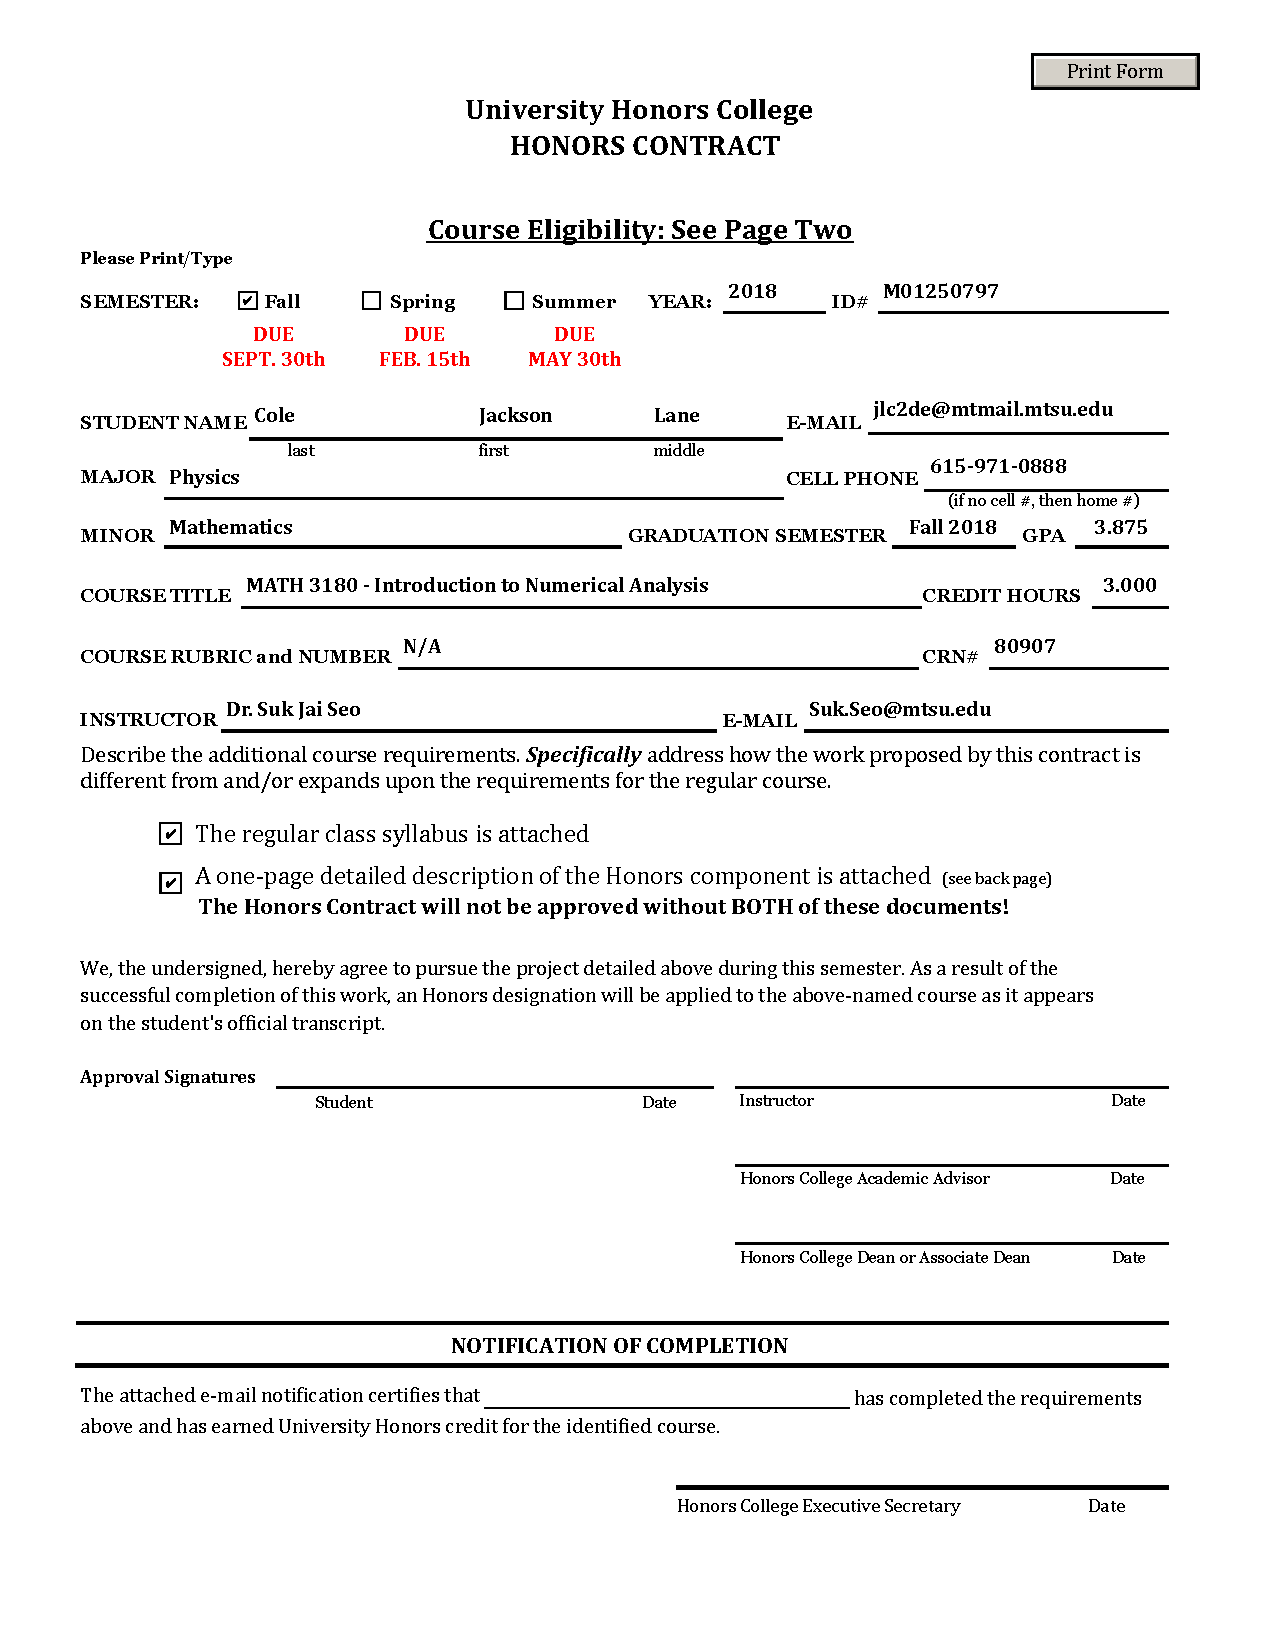
\includepdf[pages=-]{./contract_filled.pdf}
\maketitle
\tableofcontents
\listoffigures
\doublespacing

%%%%%%%%%%%%%%%%%%%%%%%%%%%%%%%%%%%%%%%%%%%%%%%%%%%%%%%%%%%%%%%%%%%%%%%%%%%%%%%%
%%%%%%%%%%%%%%%%%%%%%%%%%%%%%%%%%%%%%%%%%%%%%%%%%%%%%%%%%%%%%%%%%%%%%%%%%%%%%%%%
\section{Introduction}
When analyzing physical systems, there are often cases when analytical
solutions to ordinary differential equations describing the systems
are either exceedingly difficult to find or simply do not exist.
In these cases, it is advantageous to use numerical methods to
iteratively solve the systems. While there are several methods for solving ordinary
differential equations, the \say{workhorse} of initial value problem solvers is
the fourth-order Runge-Kutta (RK4). \cite{holmes_2018}

Essentially, the RK4 method involves computing derivatives at
four different points in the parameter space, and updating the solution at the
iterated parameter to take into account the \say{weighted average}
of the computed
derivatives. In other words, if we define a function $\functionof{f}{t, x}$, we
can say that the derivatives are calculated as shown in equation \eqref{eqn:
kderivatives}.
\begin{equation}
\begin{aligned}
    k_1 &= \functionof{f}{t_i,\, x_i}\\
    k_2 &= \functionof{f}{t_i + \frac{1}{2}h,\, x_i + \frac{1}{2}k_1}\\
    k_3 &= \functionof{f}{t_i + \frac{1}{2}h,\, x_i + \frac{1}{2}k_2}\\
    k_4 &= \functionof{f}{       t_i + h,\,        x_i + k_3}\\
    \label{eqn: kderivatives}
\end{aligned}
\end{equation}
The solution is updated
\begin{equation}
    x   = x_i + \mathbf{\frac{1}{6}}\paren{k_1 + 2k_2 + 2k_3 + k_4}h
\end{equation}
and the time is naturally updated by
\begin{equation}
    \label{eqn: time update}
    t = t_i + h.
\end{equation}
Eventually, from the given function which we assume to be the derivative of some
function of interest, the Runge-Kutta will approximate the real value of the
function of interest at some parameter. For this reason, we tend to call these
methods \say{integrators}, as they find a value for the real function of
interest when all we know is the derivative.

However, while the choice of the bolded leading coefficient seems to come
from a desire to
appropriately average the derivatives, \citet{holmes_2018} points out that
this constant is largely arbitrary, but is as standard chosen to be
$\frac{1}{6}$ to match the results of other methods. This derivation is not of
importance in the case of this project.

To be more explicit in the definition of the scheme of the RK4, we could express
it a bit differently, as shown in equation \eqref{eqn: more general rk4}.
\begin{equation}
\begin{aligned}
	k_1 &= f(t_i & + &(          0)h, &x_i& + & &           (0)k_1& + &           (0)k_2& + &           (0)k_3& + &           (0)k_4&)&\\
    k_2 &= f(t_i & + &(\frac{1}{2})h, &x_i& + & & (\frac{1}{2})k_1& + &           (0)k_2& + &           (0)k_3& + &           (0)k_4&)&\\
    k_3 &= f(t_i & + &(\frac{1}{2})h, &x_i& + & &           (0)k_1& + & (\frac{1}{2})k_2& + &           (0)k_3& + &           (0)k_4&)&\\
    k_4 &= f(t_i & + &(          1)h, &x_i& + & &           (0)k_1& + &           (0)k_2& + &           (1)k_3& + &           (0)k_4&)&\\
	x   &=       &   &                &x_i& + &[& (\frac{1}{6})k_1& + & (\frac{2}{6})k_2& + & (\frac{2}{6})k_3& + & (\frac{1}{6})k_4 &]&h\\
    \label{eqn: more general rk4}
\end{aligned}
\end{equation}
If we extract the coefficients of the step sizes, the internal
coefficients, and the weights of the derivatives in the bottom line of equation
\eqref{eqn: more general rk4}, with some abstraction, we obtain what is known
as the Butcher Tableau describing the scheme of the RK4. This is shown in Figure
\ref{fig: full rk4 butcher}. Because this is clearly just a lower triangular
matrix, we can more simply express it as in Figure \ref{fig: RK4 butcher tableau}.
It should be noted that explicit Runge-Kutta routines have the requirement
that their associated Butcher Tableau is strictly lower diagonal, as this removes
the possibility of
needing to solve implicit equations while calculating successive derivatives.
Further, a sample C++ snippet has been given for running an RK4 routine as
shown below in listing \ref{listing_RK4}.

\begin{figure}[h!]
    {\renewcommand\arraystretch{1.2}
    \begin{equation*}
        \begin{array}{ c|ccccc }
            0              & 0           & 0           & 0      &0\\
            \frac{1}{2}    & \frac{1}{2} & 0           & 0      &0\\
            \frac{1}{2}    & 0           & \frac{1}{2} & 0      &0\\
            1              & 0           & 0           & 1      &0\\
            \hline
            & \frac{1}{6} & \frac{1}{3}& \frac{1}{3}  & \frac{1}{6}\\
        \end{array}
    \end{equation*}
    \caption[Full Butcher Tableau for explicit fourth-order Runge-Kutta (RK4)] {
                Full Butcher Tableau for explicit fourth-order Runge-Kutta (RK4).
				This form comes from an abstraction of the full RK4 scheme.
            }
    \label{fig: full rk4 butcher}
    }
\end{figure}

\begin{figure}[h!]
    {\renewcommand\arraystretch{1.2}
    \begin{equation*}
        \begin{array}{ c|ccccc }
            0              &             &             &        &\\
            \frac{1}{2}    & \frac{1}{2} &             &        &\\
            \frac{1}{2}    & 0           & \frac{1}{2} &        &\\
            1              & 0           & 0           & 1      &\\
            \hline
            & \frac{1}{6} & \frac{1}{3}& \frac{1}{3}  & \frac{1}{6}\\
        \end{array}
    \end{equation*}
    \caption[Butcher Tableau for explicit fourth-order Runge-Kutta (RK4)] {
                Butcher Tableau for explicit fourth-order Runge-Kutta (RK4).
                This form of the tableau is found in many texts, so I will
                omit a reference here.
            }
    \label{fig: RK4 butcher tableau}
    }
\end{figure}

\begin{lstlisting}[language=c++, numbers=left, caption=Fourth-order Runge-Kutta (RK4),
label=listing_RK4, float=h!]
// C++
for (int i = 0; i < nSteps; i++) {
    k1 = f(t, x);
    k2 = f(t + (1/2.)*h, x + (1/2.)*k1);
    k3 = f(t + (1/2.)*h, x + (1/2.)*k2);
    k4 = f(       t + h,        x + k3);
    x  = x + h*(k1 + 2*k2 + 2*k3 + k4)/6;
    t  = t + h;
}
\end{lstlisting}

Although the Runge-Kutta method is much more accurate than lower order methods
or methods like Euler, an issue that arises in the study of physical
systems is that we are often more aware of the conditions of our system than is
our integrator. When we look at systems in celestial mechanics, like the
three-body problem that has no analytical solution, we should
acknowledge that under the assumption that the system is closed, the total
mechanical energy should remain constant. Operating with this
knowledge, the validity of the solution provided by the RK4 must be called into
question as the total energy is \textit{not} conserved over long time
integrations. \cite{holmes_2018}

When modeling physical systems, a common method of of preserving conserved
quantities is to use \textit{symplectic} integrators.
While the scope of this project does not necessarily extend
to symplectic integrators outside of the possible implementation of one for
comparison of the validity of this method, they should receive some discussion.
In general, many physical systems can be described in the Hamiltonian
formulation of mechanics; this is a far more flexible approach to mechanics than
is Newtonian or even Lagrangian formulation, especially in terms of the
generalization of coordinates and the conservation of naturally conserved
quantities. \textbf{The following derivation of the Hamitonian is based on that found in
    \citet{taylor_2005}}.

In general, we can arrive at what is known as the Lagrangian for a particular
system, which can be defined by
\begin{equation}
    \Lagr = T - U
\end{equation}
where $T$ is the kinetic energy expression for the system, and $U$ is the
potential energy expression. We also assume that the Lagrangian is a function of
$n$ generalized coordinates
\begin{equation}
    \Lagr = \paren{q_1, q_2, q_3, \dots, q_n, \dot{q}_1, \dot{q}_2, \dot{q}_3,
    \dots, \dot{q}_n} = T - U
\end{equation}
which means that in terms of the generalized coordinates, Lagrange's equations
of motion can be written as second order differential equations as
\begin{equation}
    \partialtop{\Lagr}{q_i} = \derivative{}{t}\partialtop{\Lagr}{\dot{q}_i}
    \quad\text{where}\quad
    i = [1,\dots,n]
\end{equation}
However, using the Hamiltonian approach allows us to more easily express the
equations of motion as two first order differential equations. We can define the
conjugate momentum (momenta in multiple dimensions) is expressed as
\begin{equation}
    p_i = \partialtop{\Lagr}{\dot{q}_i}
\end{equation}
Now with this defined, the Hamiltonian is defined as
\begin{equation}
    \ham = \sum_{i}^{n} p_i \dot{q}_i - \Lagr.
\end{equation}
Without derivation, the equations of motion can be expressed as
\begin{equation}
    \dot{q} = \partialtop{\ham}{p}
    \quad\quad
    \dot{p} = -\partialtop{\ham}{q}.
\end{equation}

Using these equations of motion, integration schemes can be defined that
iteratively solve the system on a symplectic manifold on which the system
is defined in the first place, which means that quantities that are conserved in
the physical system will also be conserved in the iterative solution.

%\subsection{Important Note}
%Symplecticity and geometrical integration are two
%topics about which I know \textit{very little}, but I feel as though I
%understand the idea that the solutions to Hamilton's equations lie on a
%symplectic manifold, and that symplectic integrators iteratively solve the
%system on a symplectic manifold. The underlying math is mostly enigmatic to me,
%but I feel as though implementing a standard symplectic integrator would be
%doable as long as I can find an expression for the system's Hamiltonian.



\section{Purpose}
While symplectic integrators are the go-to choice for numerically solving
systems in which a Hamiltonian can be defined, Runge-Kutta methods are still
widely used for solving physical systems as well.
Further, the Runge-Kutta method should be able to be optimized such that conserved
quantities in \textit{any} system would be respected. To be more general, in any
system in which a cost function can be defined, the hope is that a method can be
developed that improves the results on a system specific basis.
The primary directive of this project is to explore the use of evolutionary
algorithms to evolve the Butcher Tableau describing an $s$-stage Runge-Kutta
scheme to improve explicit Runge-Kutta methods
in systems in which a cost function can be defined.
In celestial mechanics, for example, the obvious examples are gravitationally bound systems in
which the energy of the system must be conserved to ensure the stability of
orbits.

A secondary goal relates to
a personal interest in multi-language projects, and this will be explored by
implementing the computationally intensive portion of this project in C++ and
wrapping it as a Python library.

\section{Methods}
\subsection{General purpose explicit Runge-Kutta algorithm}
In order to have the ability to optimize the weights, nodes, and internal coefficients of
the tableau describing a Runge-Kutta scheme, a general purpose Runge-Kutta
algorithm was developed. Without specific details about processes in
the Runge-Kutta algorithm, the general idea can be visualized in Figure
\ref{fig: generic rk flowchart}.
\begin{figure}[h!]
    \centering
    \begin{tikzpicture}[]
        \node(start) [startstop]
        {START};
        \node(inBT)[io, below = of start,]
        {$s$-stage Butcher Tableau};
        \node(processRK)[process, right = of inBT, node distance = 5cm]
        {Generic Runga-Kutta};
        \node(result) [io, right = of processRK]
        {Result};
        \node(stop) [startstop, below = of result]
        {STOP};

        \draw [arrow] (start) -- (inBT);
        \draw [arrow] (inBT) -- (processRK);
        \draw [arrow] (processRK) -- (result);
        \draw [arrow] (result) -- (stop);

    \end{tikzpicture}
    \caption[Generic Runge-Kutta algorithm]{Generic Runge-Kutta algorithm}
    \label{fig: generic rk flowchart}
\end{figure}

For this reason, a general Runge-Kutta integrator shared library
has been implemented in C++ using the Boost Python Library. This library
contains methods for iteratively solving an IVP for either a single value or for
an array of values, and does so using a Runge-Kutta scheme defined by a
general Butcher Tableau and an abstracted algorithm to process the Butcher
Tableau.

This algorithm should be flexible enough to handle any explicit Runge-Kutta
scheme that can be defined in a Butcher Tableau that is strictly
lower-triangular. For instance, the fifth order Runge-Kutta-Fehlberg method
essentially follows the general RK form, but has an extra step and is defined
by its lower-triangular Butcher Tableau.
The methods included in this library should handle the entire tableau
appropriately. While this has not been tested, there have been even higher order
Runge-Kutta schemes established ($s> 10$) in astronomical simulations that
should be able to be processed by this algorithm.

If the integrator is given the Butcher Tableau for the classic
fourth-order Runge-Kutta (RK4) as in Figure \ref{fig: RK4 butcher tableau}, the
integrator will integrate using a classic RK4 routine.
Although there are also
implicit Runge-Kutta methods that work with non-lower-triangular Butcher Tableaus,
my algorithm assumes that the matrix given is strictly lower-triangular, and
therefore, only explicit Runge-Kutta schemes can be used.


\subsection{\texttt{nbody} package}
In astronomy and astrophysics, a problem that arises in nearly every discussion
of celestial mechanics is simply known as the $n$-body problem. When two bodies
are in orbit around a common center of mass, their orbits can be described by
purely analytical functions. In other words, the motions of two orbiting
bodies have solutions that can simply be written down on paper. In the case of
systems of $n$-bodies where $n\gg2$, the solutions describing the motions of the
bodies can be approximated by cloud approaches, where each particle or star is
not analyzed individually. However, in cases where the number of bodies is
greater than two, but less than that which could be approximated by cloud
physics, an analytical solution to the $n$-body problem does not exist, and
therefore, the problem must be solved by numerical methods alone.

The initial motivation for this project was the inherent loss of energy that
occurs when iteratively solving the $n$-body problem without using a symplectic
integrator. For this reason, the method by which the general Runge-Kutta
library was going to be tested was by iteratively solving the $n$-body
problem for systems where $n < 4$. Rather than do an ad-hoc implementation of
this, a better solution supporting reproducibility of results and
simplification of the codebase was to implement \texttt{Body} and
\texttt{System} classes, where the \texttt{System} class is a system of $n$
\texttt{Body} objects. These are implemented in Python, and are now in a package
called \texttt{nbody}.

The \texttt{System} class contains methods for calculating the radii between all
bodies in the system and accelerations of all bodies due to other bodies.
The Runge-Kutta library expects to receive a name of a Python function receiving
arguments relating to the time step, the current value, and in the case of the
vector Runge-Kutta methods, the index of the current element in the array. This
allows users to write their differential equations as Python functions, which
are then called in the Runge-Kutta library.

This class also saves positions and velocities for each of the bodies in the
system, which can then be visualized after it finishes running.

Further, by creating this class, the interaction with the Runge-Kutta library
can be veiled in a simple \texttt{run} method. This then handles computation of
the gravitational forces between each pair of bodies in the system and performs
the integration at each time step.

\section{Preliminary results}
At this point, the Runge-Kutta shared library has been successfully built and
tested with several trivial first order ordinary differential equations. It
successfully accepts any lower-triangular Butcher Tableau and performs the RK
routine it defines.

Further, a $n$-body model has successfully been written in Python using the
Runge-Kutta library previously mentioned. The interface to this \texttt{nbody}
package is very simple, and requires that the user define a few bodies,
instantiate the system using a list of these bodies, and then define the
time bounds and step size to set up the RK integrators for $x$, $y$, and $z$
positions and velocities. Then the user just has to use the run method provided
to solve the system.
%A sample of the usage of these methods is given in Appendix
%\ref{app:jupyter}.

While this is now working, the results still reflect the lack of correction for
energy loss that occurs as a result of our method of integration. Basically, the
Runge-Kutta library works as expected, but returns bad solutions due to the
nature of the problem. One such solution can be seen in Figure
\ref{fig:decayingorbits}, where we simulate the Earth-Sun system. Without
correction or optimization to minimize changes in energy, the orbit of the Earth
rapidly decays in less than one revolution.
%
\begin{figure}[ht!]
    \centering
    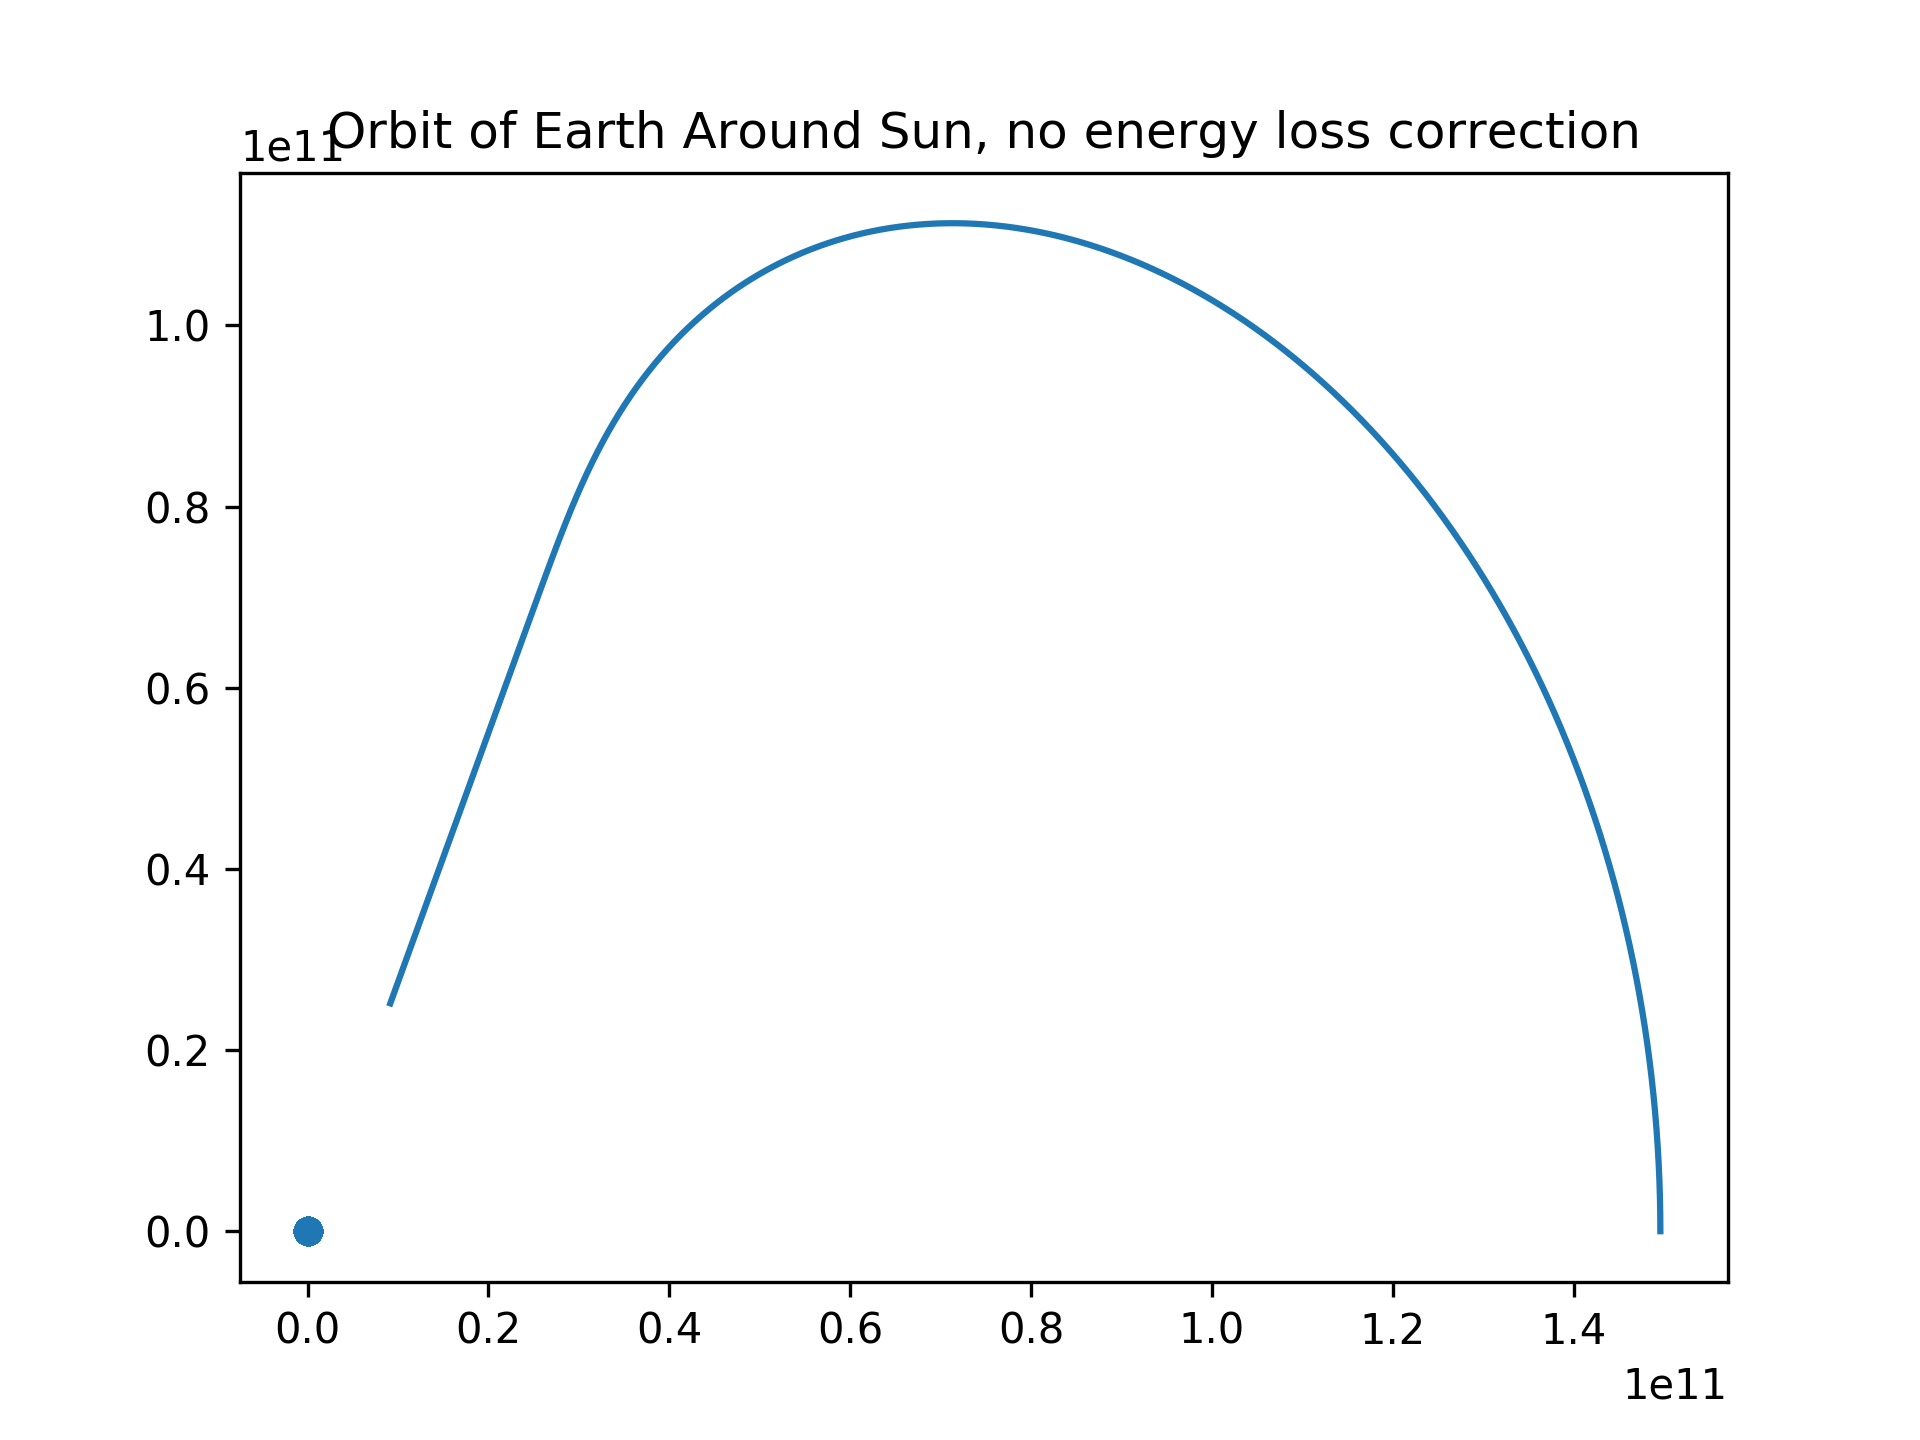
\includegraphics[width=0.5\linewidth]{images/decayingorbits.png}
    \caption{Orbital decay within one revolution of the Earth around the Sun}
    \label{fig:decayingorbits}
\end{figure}
%
This is the point at which evolutionary programming can
be used, as at this point, we operate on the assumption that the $n$-body
problem can be considered as an optimization problem for some evolutionary
algorithm, where the cost function to minimize is the energy loss.
The next steps are described in~\ref{sec:future}.


\section{Future work}\label{sec:future}
\subsection{Evolutionary algorithm to optimize variable stage Butcher Tableau using
    DEAP}

If the $n$-body simulation is carried out without any correction, the orbits
quickly decay due to energy loss. This can be seen in a simple model of the
Earth and the Sun, shown in Figure \ref{fig:decayingorbits},
where the orbit decays in less than one revolution. This is to be expected, as
we are using a non-symplectic integrator to solve a system for which solutions
exist on a symplectic manifold.

To try to programmatically reduce this error, we want to optimize the
Butcher Tableau defining the RK scheme via evolutionary algorithms.
Because we know that energy should
be conserved, the change in total energy of the system should give us a cost
function that we naturally want to minimize when evolving the Butcher Tableau.

The evolution of the Butcher Tableau will be done in Python using the DEAP
(Distributed Evolutionary Algorithms in Python) framework. This is a framework
developed \say{for rapid prototyping and testing of ideas,} and to
\say{make algorithms explicit and data structures transparent.}\cite{DEAP} This framework
provides a method to create
individuals using user-defined data types, which is helpful for quickly
generating a solution for evolving the tableaus.

Further, a common problem with evolutionary techniques and techniques in machine
learning is that while they work exceptionally well in many cases, they can
quickly become an intellectually unsatisfying black-box. The hope is that using
a dedicated evolutionary algorithm framework will allow some degree of
transparency into the actual optimization process.

The repository for the DEAP project can be found at
\url{https://github.com/DEAP/deap}.

%\subsection{Symplectic integrator for comparison}
%While I am largely unfamiliar with workhorse symplectic integrators, I found
%several that were often mentioned by \citep{geometric_numeric}. The
%implementation of one of these integrators will not necessarily be a focal point
%of this project, but having one implemented for comparison to this method
%will aid in confirming that this method works (or fails miserably).

%\section{Methods}
%Both the generic Runge-Kutta integrator and the symplectic integrator will be
%written in C++, and the genetic routine for optimizing the Butcher Tableau will
%be written in Python. C++ is undoubtedly the far better choice for performing
%potentially computationally expensive tasks, and writing the integrators in
%C++ opens up the possibility of further optimization through parallelization of
%the code. Python can handle multiprocessing through the \texttt{multiprocessing}
%package, but can only execute one thread at a time due to the Global Interpreter
%Lock. Further, despite its ease of use, Python is simply too slow to perform
%these types of iterative computations efficiently.
%
%That being said, the natural choice for writing a evolutionary algorithm
%quickly is Python. As was mentioned, DEAP \cite{DEAP} will be used for
%development of the evolutionary algorithm for this project.
%
%Clearly, this project must then be written in a way that allows a C++ RK
%implementation to be called from Python. There are several libraries that can
%aid in this process
%(Boost, ctypes). That being said, in many cases it seems that it can be
%difficult to expose C++ data structures to Python (while I have no direct source
%for this, I have heard this mentioned many times over the years), so the C++
%will likely have to be written in a largely procedural way, such that it may
%only contain the RK method itself. Any higher level structures could then be
%written in Python.
%
%At this point, further describing the methods would likely not be productive,
%as I still need to try out several ideas.


%\begin{figure}[h!]
%    \begin{equation*}
%        \begin{array}{ c|ccc }
%            c_1    & a_{11}  & \dots  & a_{1s}\\
%            \vdots & \vdots  & \ddots & \vdots\\
%            c_s    & a_{s1}  & \dots  & a_{ss}\\
%            \hline
%                   & b_{1}  & \dots & b_{s}   \\
%        \end{array}
%    \end{equation*}
%    \caption[Butcher Tableau for implicit $s$-stage Runge Kutta] {
%        Butcher Tableau for implicit $s$-stage Runge-Kutta (taken directly
%        from \citet{geometric_numeric})
%    }
%    \label{fig: implicit butcher tableau}
%\end{figure}

%j\begin{figure}[h!]
%j    \begin{equation*}
%j        \begin{array}{ c|ccccc }
%j            0      &        &        &        &\\
%j            c_2    & a_{21} &        &        &\\
%j            c_3    & a_{31} & a_{32} &        &\\
%j            \vdots & \vdots & \vdots & \ddots &\\
%j            c_s    & a_{s1} & a_{s2} & \dots  & a_{s,s-1} \\
%j            \hline
%j                   & b_{1}  & b_{2}  & \dots  & b_{s-1}   & b_{s}\\
%j        \end{array}
%j    \end{equation*}
%j    \caption[Butcher Tableau for explicit $s$-stage Runge-Kutta] {
%j                Butcher Tableau for explicit $s$-stage Runge-Kutta. This form of
%j                the tableau is found in many texts, so I will omit a reference
%j                here.
%j            }
%j\end{figure}

%\section{Progress}
%As of right now, a generic Runge-Kutta algorithm is nearly complete. It accepts
%a Butcher Tableau abstracted to a multidimensional vector of the form
%\texttt{std::vector< std::vector<double> >}, a function of the form $f =
%\functionof{f}{t, x}$, a step size, upper and lower bounds of the time
%interval, and an initial value of the function at lower bound of the interval.
%
%The program runs, but returns an incorrect solution for the ODE. Once I am able
%to remedy the issue with the Runge-Kutta routine, I can begin working on
%implementing a symplectic integrator for comparison and then wrapping the
%generic Runge-Kutta routine for interfacing with Python.

\clearpage
\bibliography{final}

\begin{appendices}
    \section{Resources and specifications}
    The repository for this project can be found at
    \url{https://github.com/jacksonlanecole/rkev}. There is a detailed README
    located here that describes how the software is built and run.

    \section{rkev Jupyter Notebook (2018-12-14 15:50)}\label{app:jupyter}
    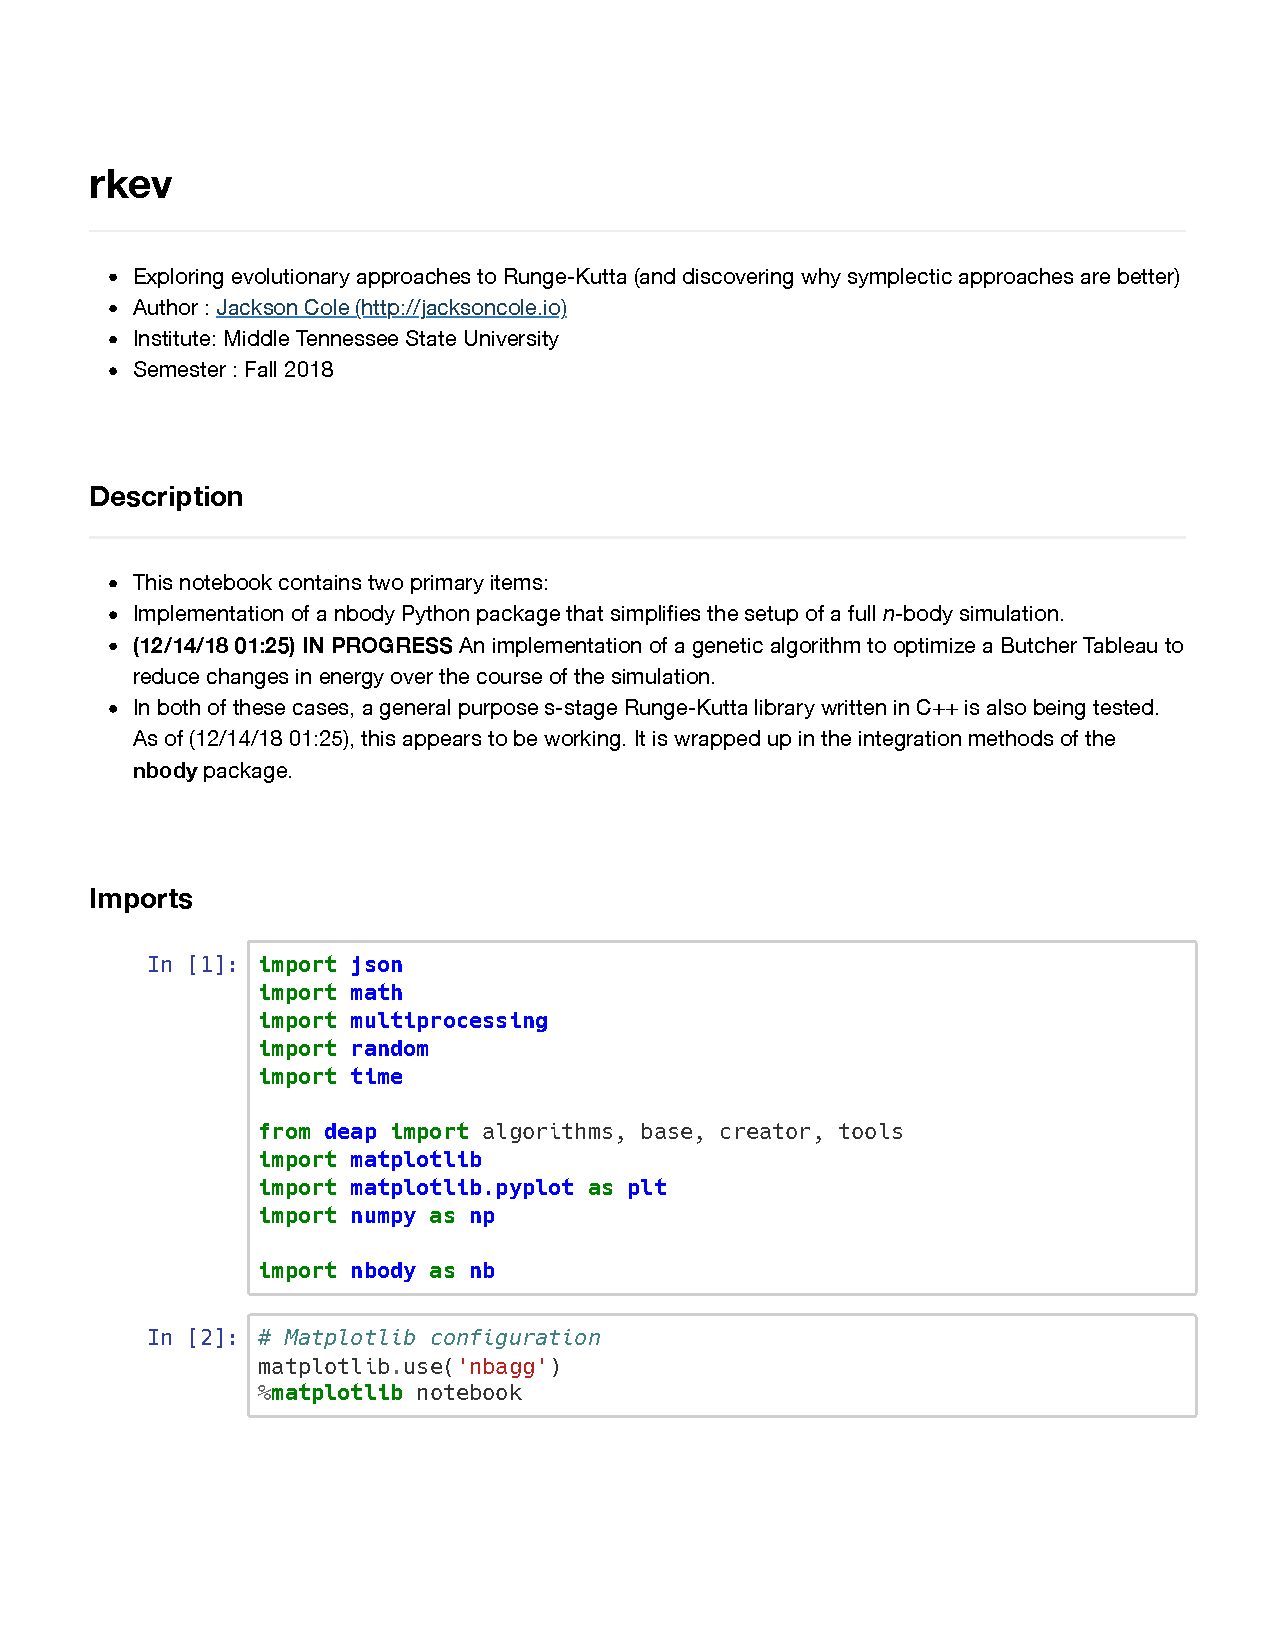
\includepdf[pages=-]{content/rkev.pdf}
\end{appendices}

%%%%%%%%%%%%%%%%%%%%%%%%%%%%%%%%%%%%%%%%%%%%%%%%%%%%%%%%%%%%%%%%%%%%%%%%%%%%%%%%
%%%%%%%%%%%%%%%%%%%%%%%%%%%%%%%%%%%%%%%%%%%%%%%%%%%%%%%%%%%%%%%%%%%%%%%%%%%%%%%%
%\partAsChapter{Time Schedule}
%\input{./content/time_schedule.tex}
%
%\partAsChapter{CV}\label{cv}
%\includepdf[pages=-]{./content/cv-jackson_cole.pdf}

\end{document}
